\documentclass{article}

\usepackage{amsmath}
\usepackage{tikz}

\def \d{2}

\begin{document}
\section{Gradient Descent}

\begin{align}
  C'(w) = \lim_{\epsilon \to 0}\frac{C(w + \epsilon) - C(w)}{\epsilon} \\
\end{align}

\subsection{``Twice''}

\begin{align}
  C(w) &= \frac{1}{n}\sum_{i = 1}^{n}(x_i w - y_i)^2 \\
  C'(w) &= \left(\frac{1}{n}\sum_{i = 1}^{n}(x_i w - y_i)^2\right)' \\
        &= \frac{1}{n}\left(\sum_{i = 1}^{n}(x_i w - y_i)^2\right)' \\
        &= \frac{1}{n}\sum_{i = 1}^{n}\left((x_i w - y_i)^2\right)' \\
        &= \frac{1}{n}\sum_{i = 1}^{n}2(x_i w - y_i)\left(x_i w - y_i\right)' \\
        &= \frac{1}{n}\sum_{i = 1}^{n}2(x_i w - y_i)x_i
\end{align}

\begin{align}
  C(w) &= \frac{1}{n}\sum_{i = 1}^{n}(x_i w - y_i)^2 \\
  C'(w) &= \frac{1}{n}\sum_{i = 1}^{n}2(x_i w - y_i)x_i
\end{align}

\subsection{One Neuron Model with 2 inputs}

\begin{center}
  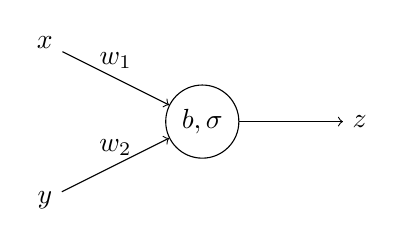
\begin{tikzpicture}
    \node (X) at (-\d, 1) {$x$};
    \node (Y) at (-\d, -1) {$y$};
    \node[shape=circle, draw=black] (N) at (0, 0) {$b, \sigma$};
    \node (Z) at (+\d, 0) {$z$};
    \path[->] (X) edge node[above] {$w_{1}$} (N);
    \path[->] (Y) edge node[above] {$w_{2}$} (N);
    \path[->] (N) edge (Z);
  \end{tikzpicture}
\end{center}

\begin{align}
  y &= \sigma(xw_{1} + yw_{2} + b) \\
  \sigma(x) &= \frac{1}{1 + e^{-x}} \\
  \sigma'(x) &= \sigma(x)(1 - \sigma(x))
\end{align}

\subsubsection{Cost}

\def \pd[#1]{\partial_{#1}}
\def \avgsum[#1, #2]{\frac{1}{#2}\sum_{#1=1}^{#2}}
\begin{align}
  a_i &= \sigma(x_{i}w_{1} + y_{i}w_{2} + b) \\
  \pd[w_{1}] a_{i} &= a_{i}(1 - a_{i}) \pd[w_{1}] (x_{i}w_{1} + y_{i}w_{2} + b) \\
                     &= a_{i}(1 - a_{i}) x_{i} \\
  \pd[w_{2}] a_{i} &= a_{i}(1 - a_{i}) y_{i} \\
  \pd[b] a_{i} &= a_{i}(1 - a_{i}) \\
  C &= \avgsum[i, n](a_{i} - z_{i})^{2} \\
  \pd[w_{1}] C &= \avgsum[i, n] \pd[w_{1}] \left( (a_{i} - z_{i})^{2} \right) \\
              &= \avgsum[i, n] 2(a_{i} - z_{i}) \pd[w_{1}] \left( a_{i} \right) \\
  \pd[w_{1}] C &= \avgsum[i, n] 2(a_{i} - z_{i}) a_{i}(1 - a_{i}) x_{i} \\
  \pd[w_{2}] C &= \avgsum[i, n] 2(a_{i} - z_{i}) a_{i}(1 - a_{i}) y_{i} \\
  \pd[b] C &= \avgsum[i, n] 2(a_{i} - z_{i}) a_{i}(1 - a_{i})
\end{align}

\subsection{Two Neurons Model with 1 input}

\begin{center}
  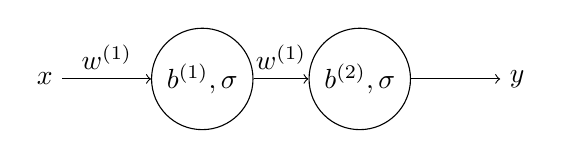
\begin{tikzpicture}
    \node (X) at (-2*\d, 0) {$x$};
    \node[shape=circle, draw=black] (N1) at (-\d, 0) {$b^{(1)}, \sigma$};
    \node[shape=circle, draw=black] (N2) at (0, 0) {$b^{(2)}, \sigma$};
    \node (Y) at (+\d, 0) {$y$};
    \path[->] (X) edge node[above] {$w^{(1)}$} (N1);
    \path[->] (N1) edge node[above] {$w^{(1)}$} (N2);
    \path[->] (N2) edge (Y);
  \end{tikzpicture}
\end{center}

\begin{align}
  a^{(1)} &= \sigma(xw^{(1)} + b^{(1)}) \\
  y &= \sigma(a^{(1)}w^{(2)} + b^{(2)}) \\
\end{align}

\subsubsection{Cost}

\begin{align}
  a_{i}^{(1)} &= \sigma(x_{i}w^{(1)} + b^{(1)}) \\
  a_{i}^{(2)} &= \sigma(a_{i}^{(1)}w^{(2)} + b^{(2)}) \\
  \pd[w^{(2)}] a_{i}^{(2)} &= a_{i}^{(2)} (1 - a_{i}^{(2)}) a_{i}^{(1)} \\
  \pd[b^{(2)}] a_{i}^{(2)} &= a_{i}^{(2)} (1 - a_{i}^{(2)}) \\
  \pd[a_{i}^{(1)}] a_{i}^{(2)} &= a_{i}^{(2)} (1 - a_{i}^{(2)}) w^{(2)} \\
  C^{(2)} &= \avgsum[i, n] (a_{i}^{(2)} - y_{i})^{2} \\
  \pd[w^{(2)}] C^{(2)} &= \avgsum[i, n] \pd[w^{(2)}] \left( (a_{i}^{(2)} - y_{i})^{2} \right) \\
                 &= \avgsum[i, n] 2 (a_{i}^{(2)} - y_{i}) \pd[w^{(2)}] \left( a_{i}^{(2)} \right) \\
                 &= \avgsum[i, n] 2 (a_{i}^{(2)} - y_{i}) a_{i}^{(2)} (1 - a_{i}^{(2)}) a_{i}^{(1)} \\
  \pd[b^{(2)}] C^{(2)} &= \avgsum[i, n] 2 (a_{i}^{(2)} - y_{i}) a_{i}^{(2)} (1 - a_{i}^{(2)}) \\
  \pd[a_{i}^{(1)}] C^{(2)} &= \avgsum[i, n] 2 (a_{i}^{(2)} - y_{i}) a_{i}^{(2)} (1 - a_{i}^{(2)}) w^{(2)} \\
\end{align}

using the chain rule that:

\begin{align}
  \pd[w^{(1)}] C^{(2)} &= \avgsum[i, n] \pd[a_{i}^{(1)}] C^{(2)} \cdot \pd[w_{(1)}] a_{i}^{(1)} \\
                       &= \avgsum[i, n] \pd[a_{i}^{(2)}] C^{(2)} \cdot \pd[a_{i}^{(1)}] a_{i}^{(2)} \cdot \pd[w_{(1)}] a_{i}^{(1)}
\end{align}

so we can use the $\pd[a_{i}^{(1)}] C^{(2)}$ to move backwards.

but before that, we need to define the ``Cost'' of the fist layer

\begin{align}
  a_{i}^{(1)} &= \sigma(x_{i}w^{(1)} + b^{(1)}) \\
  \pd[w^{(1)}] a_{i}^{(1)} &= a_{i}^{(1)} (1 - a_{i}^{(1)}) w^{(1)} \\
  e_{i} &= a_{i}^{(1)} - \pd[a_{i}^{(1)}] C^{(2)} \\
  C^{(1)} &= \avgsum[i, n] (a_{i}^{(1)} - e_{i})^{2} \\
  \pd[w^{(1)}] C^{(1)} &= \pd[w^{(1)}] \left( \avgsum[i, n] (a_{i}^{(1)} - e_{i})^{2} \right) \\
                       &= \avgsum[i, n] \pd[w^{(1)}] \left( (a_{i}^{(1)} - e_{i})^{2} \right) \\
                       &= \avgsum[i, n] 2 (a_{i}^{(1)} - e_{i}) \pd[w^{(1)}] \left( a_{i}^{(1)} \right) \\
                       &= \avgsum[i, n] 2 (\pd[a_{i}^{(1)}] C^{(2)}) x_{i} \\
  \pd[b^{(1)}] C^{(1)} &= \avgsum[i, n] 2 (\pd[a_{i}^{(1)}] C^{(2)})
\end{align}

note that this is literally the same as to make it out with chain rule, but it's easier to code in this way.

\subsection{Arbitrary Neurons Model with 1 input}

\begin{center}
  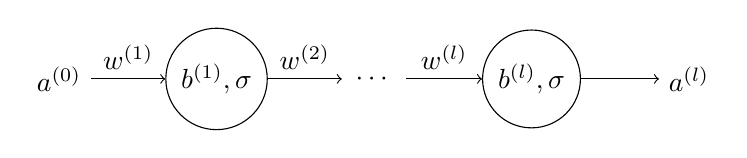
\begin{tikzpicture}
    \node (X) at (-2*\d, 0) {$a^{(0)}$};
    \node[shape=circle, draw=black] (N1) at (-\d, 0) {$b^{(1)}, \sigma$};
    \node[shape=circle] (N2) at (0, 0) {$\cdots$};
    \node[shape=circle, draw=black] (N3) at (\d, 0) {$b^{(l)}, \sigma$};
    \node (Y) at (+2*\d, 0) {$a^{(l)}$};
    \path[->] (X) edge node[above] {$w^{(1)}$} (N1);
    \path[->] (N1) edge node[above] {$w^{(2)}$} (N2);
    \path[->] (N2) edge node[above] {$w^{(l)}$} (N3);
    \path[->] (N3) edge (Y);
  \end{tikzpicture}
\end{center}

\subsubsection{Feed-Forward}

\begin{align}
  a_{i}^{(j)} &= \sigma(a_{i}^{(j-1)}w^{(j)} + b^{(j)}) \\
  \pd[w^{(j)}] a_{i}^{(j)} &= a_{i}^{(j)} (1 - a_{i}^{(j)}) a_{i}^{(j-1)} \\
  \pd[b^{(j)}] a_{i}^{(j)} &= a_{i}^{(j)} (1 - a_{i}^{(j)}) \\
  \pd[a_{i}^{(j-1)}] a_{i}^{(j)} &= a_{i}^{(j)} (1 - a_{i}^{(j)}) w^{(j)}
\end{align}

\subsubsection{Back-Propagation}

\begin{align}
  e_{i}^{(j)} &= a_{i}^{(j)} - \pd[a_{i}^{(j)}] C^{(j+1)} \\
  C^{(j)} &= \avgsum[i, n] (a_{i}^{(j)} - e_{i}^{(j)})^{2} \\
  \pd[w^{(j)}] C^{(j)} &= \pd[w^{(j)}] \left( \avgsum[i, n] (a_{i}^{(j)} - e_{i}^{(j)})^{2} \right) \\
                       &= \avgsum[i, n] \pd[w^{(j)}] \left( (a_{i}^{(j)} - e_{i}^{(j)})^{2} \right) \\
                       &= \avgsum[i, n] 2 (a_{i}^{(j)} - e_{i}^{(j)}) \pd[w^{(j)}] \left( a_{i}^{(j)} \right) \\
                       &= \avgsum[i, n] 2 (\pd[a_{i}^{(j)}] C^{(j+1)}) a_{i}^{(j)} (1 - a_{i}^{(j)}) a_{i}^{(j-1)} \\
  \pd[w^{(j)}] C^{(j)} &= \avgsum[i, n] 2 (\pd[a_{i}^{(j)}] C^{(j+1)}) a_{i}^{(j)} (1 - a_{i}^{(j)}) \\
  \pd[a_{i}^{(j-1)}] C^{(j)} &= \avgsum[i, n] 2 (\pd[a_{i}^{(j)}] C^{(j+1)}) a_{i}^{(j)} (1 - a_{i}^{(j)}) w^{(j)}
\end{align}

\end{document}
